
\newacronym{ma}{MA}{Manufactura Aditiva}
\newacronym{fdm}{FDM}{Manufactura asistida por computadora}
\newacronym{iot}{IoT}{Internet de las cosas}
\newacronym{m2m}{M2M}{machine two machine}
\newacronym{ASTM}{ASTM}{American Society for Testing and Materials}

\newacronym{pyme}{PyME}{Pequeña y mediana empresa}

\printglossary[type=\acronymtype]


\newpage
\begin{multicols}{2}
\nomenclature{$d$}{diametro}
\nomenclature{$m$}{Masa}
\nomenclature{$l$}{Carga Aplicada}
\nomenclature{$P$}{Paso del Tornillo}
\nomenclature{$I_p$}{Inercia Plataforma}
\nomenclature{$I_t$}{Inercia Tornillo}
\nomenclature{$I_{eq}$}{Inercia Equivalente}
\nomenclature{$T_a$}{Torque para mover el sistema}
\nomenclature{$T_b$}{Torque para vencer fuerza fricción}
\nomenclature{$T$}{Torque Total}
\nomenclature{$V_{max}$}{Velocidad Maxima}
\nomenclature{$F_f$}{Fuerza de Fricción}
\nomenclature{$e{ff}$}{Eficiencia}
\nomenclature{$\sigma_{Max}$}{Esfuerzo Máximo}
\nomenclature{$S_y$}{Resistencia a la Fluencia del Material}
\nomenclature{$I$}{Inercia}
\nomenclature{$V_c$}{Cortante}
\nomenclature{$A$}{Área}
\nomenclature{$A$}{Base}
\nomenclature{$h$}{Altura}
\nomenclature{$sps$}{Altura}
\nomenclature{$spr$}{Altura}
\nomenclature{$M$}{Momento Flector}
\nomenclature{$Fr$}{Fuerza de Rozamiento}
\nomenclature{$g$}{Gravedad}
\nomenclature{$Dp$}{Distancia Poleas}
\nomenclature{$V$}{Velocidad}
\nomenclature{$F_n$}{Fuerza Normal}
\nomenclature{$F$}{Fuerza}
\nomenclature{$\sigma_d$}{Esfuerzo de Diseño}
\nomenclature{$S_y$}{Modulo de Young}
\nomenclature{$n$}{Factor de seguridad}
\nomenclature{$\sigma '$}{Esfuerzo de Fluencia}






\printnomenclature
\end{multicols}
\clearpage %poner esta linea al inicio de cada capitulo
\chapter{Introducción}

La tecnología de manufactura aditiva ha tomado gran importancia en el campo ingenieril, esto se debe a las ventajas que proporciona. Por mencionar algunas de ellas ,se encuentra la facilidad en la realización de figuras con geometrías abstractas y la posibilidad de personalizar los diseños, esta ha sido una de las  razones, por la que muchas empresas están interesadas en manejar este tipo de tecnología, permitiendo lograr a nivel mundial un gran auge. En consecuencia, actualmente la \acrshort{ma} está inmersa en el área aeroespacial, médica y automotriz, posicionándola en el mercado como novedosa y atractiva. \cite{moleon}\\

Para contextualizar la \acrshort{ma} como lo expresa \cite{heinze} \textit{“Es una técnica que permite la producción de modelos a partir de imágenes bidimensionales con la ayuda de un software   especializado   y   una   impresora   3-D”}. \cite{blaquez}  explica que la técnica parte del principio de lo que se conoce como impresión aditiva; en la que el objeto deseado se construye depositando múltiples capas de material una encima de la otra. Se trata de un proceso altamente especializado capaz de convertir imágenes digitales en modelos físicos que pueden tener diversos usos. \\


\cite{chen} expresa que la adopción de esta tecnología en la actualidad se ha intensificado, por su capacidad de evolución ya que en un principio “los modelos solían estar hechos de materiales rígidos y carecían de realismo y detalles anatómicos, pero la introducción de nuevas materias primas ha permitido crear modelos de materiales más elásticos similares al tejido humano que,con la adición de colores y otros detalles, han dado lugar a modelos con un gran realismo” .Es indispensable destacar otra ventajas, como las encontradas en la investigación de \cite{reyes}, el cual demuestra que al utilizar este tipo de tecnología se evidencia reducción en los costos de producción, disminución de tiempos, protección del medio ambiente a través del reciclaje, versatilidad y personalización. \\


Esta tecnología actualmente cuenta con la deficiencia que no se ha explotado toda su capacidad, en la integración con otros protocolos de comunicación, lo que daría paso a mejorar su interoperabilidad y un manejo intuitivo por personas que no posean ningún tipo de conocimiento en \acrshort{ma}.Teniendo en cuenta estas deficiencias se propone realizar una integración de la maquina v-make con \acrshort{iot}, el cual tiene como función interconectar billones de objetos entre sí a través de Internet, con la finalidad de que exista una comunicación máquina-máquina, dónde todos ellos podrían ser visibles e interaccionar.\\

\citep{reyes} expresa que las aplicaciones son casi infinitas y actualmente está enfocado en su mayoría en la domótica ,algunos de sus usos cotidianos son el control del tráfico, el control de los suministros de agua , calefacción en un edificio,  control de transporte público, etc.\\ %cristian

Teniendo en cuenta estos dos grandes temas y el aporte que se puede generar en la unificación de estas tecnologías, se propone la construcción de una máquina  de fabricación aditiva con integración \acrshort{iot}. 




\section{Antecedentes}  \label{antecedentes}

\citep{blaquez} realiza una breve introducción en la definición de \acrshort{ma}, explica que este tipo de manufactura, se basa en producir objetos a través de la adición de material en capas siguiendo como patrón informaciones numéricas representadas en código, que permiten la creación del objeto deseado, mediante el diseño y conexion de distintas areas en un mismo proceso .\\

Para el proceso de adición se utiliza la tecnología \acrshort{fdm} mostrada en la \autoref{fig:FDM},la cual consiste en \textit{“ desenrollar un filamento de plástico de una bobina y abastecer
el material hacia una boquilla de extrusión, la boquilla se
alimenta con el filamento que es calentado a una temperatura
por debajo de la temperatura de fusión del material. La boquilla
deposita una fina capa de plástico una encima de otra hasta
terminar completamente la pieza. El material fundido se
solidifica al ir haciendo contacto con la superficie donde el
material se va uniendo para obtener un sólido.''}\citep{acuna} 

\begin{figure}[H]
    \centering
    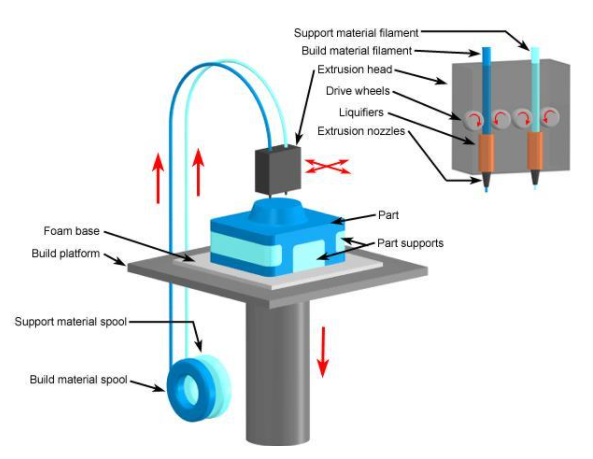
\includegraphics[width=0.5\textwidth]{Figs/FDU.PNG}
    \caption{FDM, \citep{blaquez}}
     \label{fig:FDM}
\end{figure}

Complementando esta información en el libro de \citep{berchon} se muestras algunas operaciones relacionadas con la impresion 3D y las partes que componen la misma \autoref{fig:IMP3D}. \\

\begin{itemize}
  \item Extrusión- Modelado por deposición fundida
  \item Hilado-Fabricación por haz de electrones
  \item Granulado-Sinterizado por calor o laser
  \item Laminado-Laminado de capas
  \item Fotoquímicos-Fotopolimerización por luz ultravioleta
\end{itemize}

\begin{figure}[H]
    \centering
    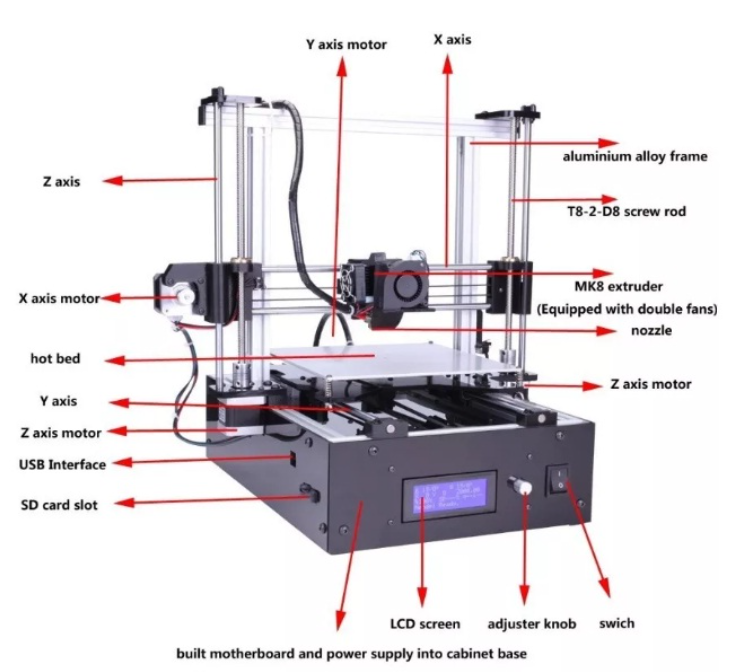
\includegraphics[width=0.8\textwidth]{Figs/partes.PNG}
    \caption{Partes Impresión 3D}
    \textbf{Fuente:\:https://www.itekmiv.com/p/impresora-3d-frame-aluminio/}
     \label{fig:IMP3D}
\end{figure}

Teniendo en cuenta estos detalles, \citep{muller} demuestra que la manufactura aditiva tiene grandes ventajas sobre la manufactura convencional enfocándose principalmente en piezas pequeñas.  Afirma en su estudio que este tipo de tecnología \textit{‘‘permite modificar las cosas de manera sencilla y rediseñar los elementos sin necesidad de gastar tanto material de esta manera ahorra mucho dinero. Los beneficios son una cantidad mínima de sujeción, piezas más precisas y menos horas de producción’’}.  \\


Pese a los beneficios que tiene en relación a otros procesos de construcción, la impresión 3D no está independiente de problemas o inconvenientes.\citep{alvarez} expresa que \textit{''una de las principales problemáticas se presenta al momento de configurar una impresión,determinando los parámetros adecuados. En ocasiones, la elección se realiza en función de la experiencia de los operadores, pero cuando se requieren propiedades específicas, no se conocen los parámetros a elegir.''} \\

Indagando mas problemáticas y a partir de la experiencia en el uso de estas maquinas de bajo costo, se encuentran problemas relacionados con el área de impresión, la falta de resistencia del material y la poca precisión en la construcción de agujeros debido a la estabilidad de la maquina.\\

Teniendo en cuenta estos datos se expone en la \autoref{fig:tipos}, algunas de las distribuciones mas comunes en las impresoras 3D.\\

\begin{figure}[H]
    \centering
    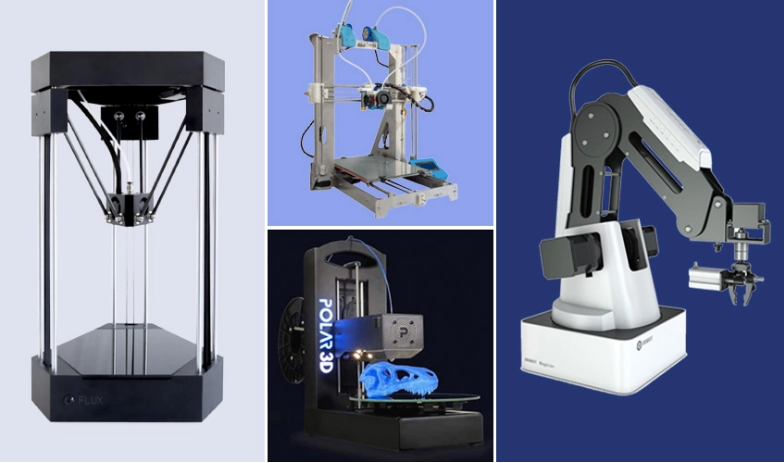
\includegraphics[width=0.8\textwidth]{Figs/tipos.PNG}
    \caption{Distribuciones impresora 3d \citep{} }
     \label{fig:tipos}
\end{figure}


Basados en los errores que se presentan en la \acrshort{ma} y la poca investigación en el contexto colombiano, se puede presentar una reducción considerable a partir de la integración de \acrshort{iot} en el proceso, ya que se obtiene mayor control en la construcción de una pieza, logrando así identificar errores y actuar de manera inmediata. por lo cual la manufactura aditiva se debe dar dentro del contexto del nuevo panorama Industrial 4.0, ‘‘donde la interoperabilidad de los sistemas de manufactura computarizados y la transparencia de la información generada, intercambiada y usada para fabricar un producto juegan un rol preponderante.’’ \citep{rodriguez} \\


A partir de la idea fundamental expresada por \citep{rodriguez} y \citep{muller} de sistemas intuitivos y de gran capacidad acorde a la industria 4.0, se encuentra la implementación de la tecnología \acrshort{iot} en distintos proyectos, uno de ellos es de la “ domótica o Home Automation, es una de las aplicaciones de Internet de las cosas más populares en el mundo , a tal punto que muchas empresas brindan soluciones para este tema, comercialmente se ofrecen bastantes dispositivos, de diferentes marcas lo que le permite tener al usuario opciones a elegir" \citep{tinoco}.\\

En la actualidad la aplicación de IoT con base en la domótica, disminuye los esfuerzos e incrementa la tranquilidad de las personas. Para entender los proceso que realizan estos sistemas \citep{fernandez} propone la siguiente comparación \textit{“ Al igual que el ser humano recibe información del medio ambiente, mediante
los sentidos, luego con esa información toma decisiones para adaptarse, así mismo funciona un sistema domótico, que mediante los dispositivos inteligentes integrados, pude recolectar la información, almacenarla y con esto tomar decisiones según las configuraciones que se realizen"}.\\

La implementación de esta aplicación de \acrshort{iot} se muestra en la \autoref{fig:domotica}

\begin{figure}[H]
    \centering
    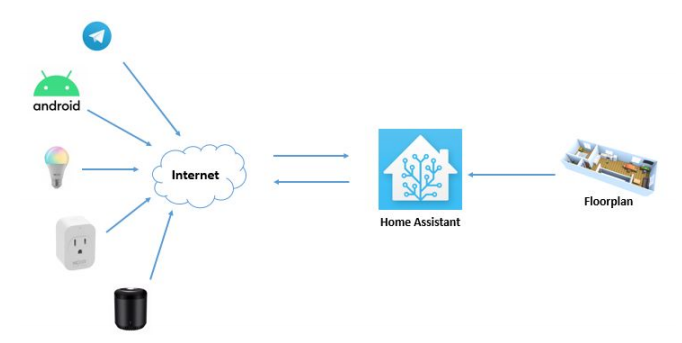
\includegraphics[width=0.8\textwidth]{Figs/iot.PNG}
    \caption{Estructura del sistema domótico \citep{tinoco} }
     \label{fig:domotica}
\end{figure}


A partir de la explicación de \acrshort{iot} , es de vital importancia,dar una introducción al protocolo u aplicación que se va a ha trabajar para su desarrollo en el proyecto.\\

OctoPrint es una aplicación de código abierto gratuita, diseñada para el control de impresoras 3D. Posibilita administrar cada una de de las impresiones de manera remota y mantener un control general siendo esta su función principal.Por lo cual, \citep{mp} afirma que el objetivo de su proyecto es “imprimir diseños
de forma remota y supervisar aspectos de la impresora 3D mediante una
Computadora.'' Explica que realiza la implementación a través de una Raspberry Pi, donde carga la información, permitiéndole así impresiones de forma remota, control de temperatura de extrucción, apagar y encender la impresora , verificar el estado de las impresiones y observarlas a través de una transmisión de vídeo en tiempo real .Afirma que estos son solo alguna de las posibilidades que se obtienen al implementar este protocolo de comunicación ya que las posibilidades son infinitas.  Al realizar la implementación del programa, se consigue una comunicación \acrshort{m2m} lo que permitiría un uso adecuado del internet de las cosas. Una de las razones por las cuales se utiliza esta aplicación, es la manera en que esta distribuida su interfaz, se puede observar en la \autoref{fig:octo} que su visualización es muy intuitiva, dándole facilidad al usuario en su uso.


\begin{figure}[H]
    \centering
    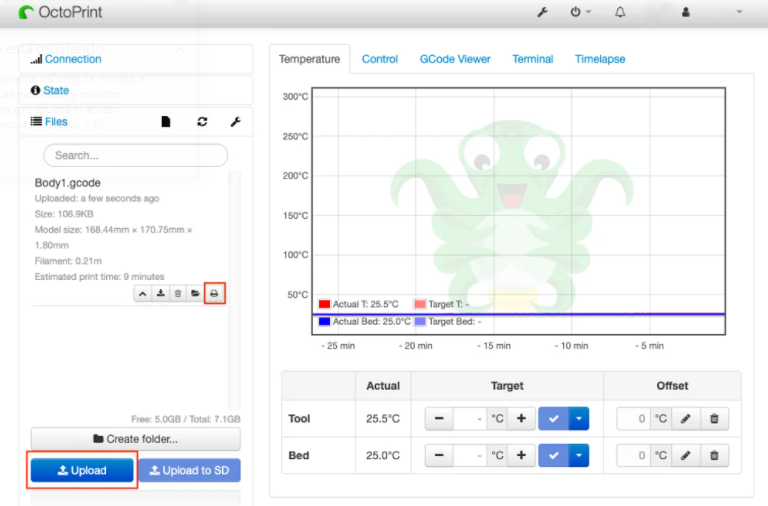
\includegraphics[width=0.8\textwidth]{Figs/octoprint.PNG}
    \caption{Interfaz OctoPrint\citep{} }
     \label{fig:octo}
\end{figure}

Finalmente cabe destacar que en el contexto colombiano la industria 4.0 no han tenido un gran desarrollo.Se encuentra que desde el año 2016 se empezó la investigación y desarrollo de la \acrshort{fdm}, la cual consistió en un proyecto conformado por un grupo interdisciplinario, que tenia como objetivo la construcción de una impresora 3d que pudiera realizar objetos a escala real. REFERENCIA\textit{ '' se cumplió con los objetivos propuestos, brindando una maquina funcional y eficiente en la construcción de piezas de gran escala''}. Este avance que se genero ,impulso la  construcción del primer modulo habitacional, en la región de medellin, mediante una mezcla de concreto como material de deposición, se consiguió la elaboración y entrega del proyecto.\\

Estos resultados causaron un boom, lo que permitió que las personas se adentraran en esta área,comenzando así el proceso de importación y distribución de impresoras 3d de gama baja y media . Aunque en comparación de los avances que se le ha dado a esta tecnología en todo el mundo es muy poco, actualmente se le esta dando importancia a la investigación y desarrollo por entes privados, ya que conocen que somos un país con una alta demanda de prótesis, viendo así un mercado con un futuro prometedor.\\

Destacando otra de las tecnologías emergentes de esta industria, en Colombia el \acrshort{iot} ha sido una de las implementaciones mas recientes y en las cuales las grandes compañías ven una tecnología, innovadora y necesaria de cara al futuro. Esto se debe a las prestaciones y facilidades que brinda en la producción.Aunque se han presentado algunas implementaciones de esta tecnología mostrando excelentes beneficios y ganancias.\citep{}REFERENCIA afirma que \textit{“Colombia tiene un marco legal que obstaculiza la apropiación de tecnologías, la transformación digital y la productividad.Considera que el desafío es cambiar la mentalidad de algunos de los principales actores, como el Gobierno, los empresarios y la academia, de manera que el país realice cambios disruptivos en todos los modelos de negocio.''}\\

Ademas \citep{}REFERENCIA complementa que \textit{“ reducir las barreras a la inversión en tecnologías digitales; adoptar marcos tecnológicos neutrales que promuevan la competencia; establecer estándares técnicos globales que permitan la interoperabilidad y un internet seguro, estable, abierto y accesible, y aumentar la velocidad de Internet. De lo contrario, se verá limitada la adopción del big data, el alojamiento de datos en la nube, el uso de inteligencia cognitiva y otras tecnologías emergentes.''}\\

\newpage
\section{Planteamiento del Problema}\label{planteamiento}

Las problemáticas por enfrentar se determinan dada la limitación en el área del trabajo, la poca estabilidad de la máquina debido a su diseño y la interoperabilidad que tiene el usuario, para controlar los procesos en tiempo real . \\

A partir de las conclusiones de \citep{rodriguez} y \citep{fernandez}, en las cuales exponen aspectos y mejoras que consideran relevantes,apoyados en fundamentaciones y avances en distintas áreas del proyecto. Se logra comprender, que la parte de diseño y construcción, para el desarrolló de la maquina esta avanzada, ya que se cuenta con una base considerable de cálculos, que permiten escoger los mejores elementos para la construcción del dispositivo. En la parte de programación y control es necesario realizar un planteamiento propio ya que cada maquina es diferente y la unificación de distintos componentes, requieren nuevas pruebas para determinar la funcionalidad .El apoyo en esta área se da a través de ejemplos de código el cual es de acceso libre, incluyendo librerías y algunos métodos de implementación.\\ 

En la revisión de la literatura ahí un tema que es común denominador, la elección de la distribución, ya que concuerdan que debe estar basada en el funcionamiento que se le va a dar al equipo.Recordando algunas de las distribuciones mas comunes, se encuentran Delta, Cartesiana, Polar y Brazo Robótico, las cuales se pueden observar en la \autoref{fig:tipos}.\\

Otro aspecto que cabe mencionar, es la necesidad de implementar los nuevos protocolos de comunicación de la industria 4.0,esto se debe a que actualmente existe la necesidad de que las maquinas posean  gran conectividad,interoperabilidad,además de la característica de ser intuitivas para el usuario, brindando así una gran experiencia en el desarrollo de cualquier proyecto.\\

A partir de la información expuesta, se propone en el desarrollo estructural de la maquina,combinar el movimiento cartesiano y de la base de trabajo, añadiendo un doble soporte en la parte posterior, lo que permitiría mayor estabilidad y precisión, las cuales son fundamentales a la hora de realizar el proceso de impresión 3D. La implementación de la tecnologías emergentes,se logra con el programa Octoprint que genera un sinfín de aplicaciones en función de la interoperabilidad de la maquinaria.\\

\newpage
\section{Justificación y pregunta de Investigación}

Se pretende viabilizar la construcción de una maquina de impresión 3D con integración \acrshort{iot}, que sea equiparable al rango de impresoras 3D básicas existentes en el mercado. Se aplica esta segmentación de mercado ya que conocemos las necesidades de primera mano de los estudiantes, en la elaboración y construcción de un proyecto que necesite procesos de manufactura.\\

 Estas razones además de los costos elevados en la adquisición de materiales y la necesidad de la optimización del tiempo en los proyectos, son los problemas mas grandes que se presentan en la construcción de piezas por manufactura tradicional.

Es de vital importancia resaltar que en el contexto colombiano, desde el 2016 ha tenido una adopción lenta y con un marco legal que no favorece como se expone en la sección \ref{antecedentes} , el desarrollo en distintas áreas es reducido y de difícil acceso debido a sus costos en el país .Aunque se cuentan con estos problemas, actualmente existe la ventaja del acceso libre a la información en un panorama mundial, lo que facilita su construcción, ya que en el mundo, “esta revolución en la manufactura de piezas ha abarcado muchas áreas, desde la ingeniería hasta la medicina, trayendo como garantía un avance hacia nuevos conocimientos. Hoy se tiene la posibilidad de re-transformar los bits en átomos, es decir: en objetos físicos, en las casas, en los talleres o en una \acrshort{pyme}, gracias a las impresoras 3D y a las máquinas de prototipado rápido''\citep{berchon}.\\

  Por lo cual se propone ofrecer una maquina que brinde presición, confianza y facilidad de operación a su usuario . Esto se logra a través de una herramienta que incluya mayor área de impresión, estabilidad y un proceso de fabricación que brinde confiabilidad. Algunos de los beneficios adicionales que se presentan es la integración con IoT,que pretende, proporcionar mayor control y supervisión en el proceso de prototipado rápido , ya que a partir de esta unificación se tiene la capacidad de controlar los procesos en tiempo real, permitiendo así una reducción en los fallos de operación existentes.\\

A raíz de lo anterior surgen las siguientes preguntas:
\begin{itemize}
\item ¿ Cuales son los factores primordiales que viabilizan la construcción y futura comercialización de la maquina descrita?
	\item ¿Cuales son los beneficios que traería la integración con IOT en el diseño de este proyecto?
	\item ¿Es posible realizar un proceso de manufactura en poco tiempo a bajo costo y con buena calidad?
\end{itemize}


\section{Objetivos}

\subsection{Objetivo General}

\begin{itemize}
	\item Implementar una máquina de impresión 3d existente en la cual se integre las técnicas de impresión 3D y CNC, con la cualidad de ser operada remotamente.
\end{itemize}

\subsection{Objetivos Específicos}
\begin{itemize}
	\item Determinar los requerimientos técnicos del sistema mecatrónico que cumpla las especificaciones de la operación deseada.
	\item Sintetizar los elementos que integran la operación de las dos tecnologías en un solo sistema. 
	\item Verificar la operación y precisión de la máquina realizando un benchmark con otras tecnologías.
\end{itemize}



\section{Métodos}



La metodología empleada fue la investigación empírico-analítica, ya que el proyecto se basa en una fundamentación teórica de conclusiones obtenidas por otros autores, la parte empírica se ve en el trabajo de dar aseveraciones teóricas de la fundamentación, por medio de experimentos.Teniendo como objetivo dar una solución a una necesidad que surge en el ámbito académico.\\

De esta manera se proporciona información confiable y practica que permite respaldar el correcto funcionamiento del modelo, verificando las ventajas propuestas en el prototipo. Esta metodología proporciona parámetros convenientes en la construcción y análisis para próximos proyectos. Teniendo en cuenta las ventajas que nos proporciona, es necesario determinar análisis confiables que incluyan las variables necesarias para una buena fundamentación, por tal motivo se desarrollo:\\


Un despliegue de función de calidad (QFD) el cual se basa en los requerimientos o demandas del usuario en la calidad del diseño. \ref{fig:QFD}. Además de la construcción de un benchmark que permita hacer una comparación entre las tecnologías existentes, obteniendo así información relevante en cuanto a especificaciones, ventajas, desventajas y costos actuales. \ref{fig:bench}. Dando paso a su construcción y desarrollo de los objetivos planteados.\\


Para su construcción, se brindo una sustentación matemática y experimental,que da un soporte confiable a la investigación, por lo cual se desarrollara, el diseño mecánico en la \autoref{mecanico} y de control en la \autoref{Dicontrol}. Teniendo como base esta sustentación, es de vital importancia, tener una referencia experimental de la calidad que se esta ofreciendo con el dispositivo, por tal motivo se implementa la norma \acrshort{ASTM} D638 y \acrshort{ASTM} D5379 ,la cual proporciona información real de las características mecánicas en los diseños realizados. En la sección \ref{norma} se dará una explicación del desarrollo general de la prueba.


